%==============================================================================
% Document header
%==============================================================================
\documentclass[a4paper,11pt]{article}

% Color package
\usepackage[usenames,dvipsnames]{color}

% Appendix package
\usepackage[toc,page]{appendix}

% Hyperrefs
\usepackage[
  colorlinks = true,
  linkcolor  = Mahogany,
  citecolor  = Mahogany,
  urlcolor   = blue,
]{hyperref}

\usepackage{graphicx}
\usepackage{multirow}


\usepackage[toc,page]{appendix}

% Header and footer customization
\usepackage{fancyhdr}
\setlength{\headheight}{15.2pt}
\pagestyle{fancy}
\fancyhead[L]{\nouppercase{\leftmark}}
\fancyhead[R]{} 
\renewcommand{\footrulewidth}{0.4pt}

%==============================================================================
% Start of document
%==============================================================================
\begin{document}

%------------------------------------------------------------------------------
% Title
%------------------------------------------------------------------------------
\begin{titlepage}

\vspace*{3cm}

\noindent{\LARGE \textbf{I$^2$C Slave Core}}

\noindent \rule{\textwidth}{.1cm}

\hfill\today

\vspace*{3cm}

\begin{figure}[h]
  
\includegraphics[height=3cm]{fig/cern-logo}
  \hfill
  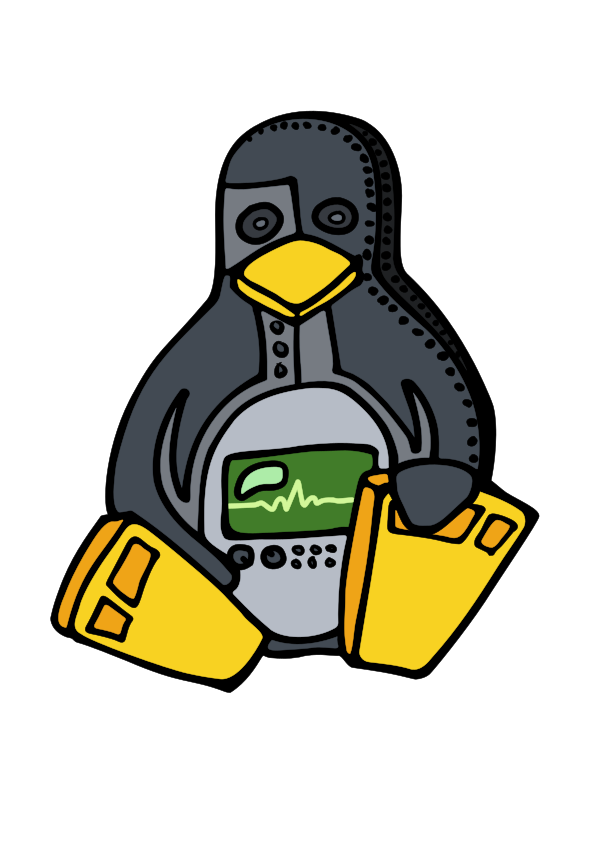
\includegraphics[height=3cm]{fig/ohwr-logo}
\end{figure}

\vfill

\noindent {\Large \textbf{Theodor-Adrian Stana (CERN/BE-CO-HT)}}

\noindent \rule{\textwidth}{.05cm}

\end{titlepage}


%------------------------------------------------------------------------------
% Revision history
%------------------------------------------------------------------------------
\thispagestyle{empty}
\section*{Revision history}

\centerline
{
  \begin{tabular}{l c p{.6\textwidth}}
  \hline
  \multicolumn{1}{c}{\textbf{Date}} & \multicolumn{1}{c}{\textbf{Version}} & \multicolumn{1}{c}{\textbf{Change}} \\
  \hline
  26-06-2013 & 0.01 & First draft \\
  14-08-2013 & 0.02 & Second draft \\
  22-10-2013 & 0.03 & Added \textit{Access commands} section, updated document according to
                      changes in protocol \\
  29-10-2013 & 0.04 & Changed PDF link colors \\
  18-12-2013 & 1.00 & Finite version with watchdog timer and robust communication \\
  \hline
  \end{tabular}
}

\pagebreak
\pagenumbering{roman}
\setcounter{page}{1}
\tableofcontents

%------------------------------------------------------------------------------
% List of figs, tables, abbrevs
%------------------------------------------------------------------------------
\pagebreak
\listoffigures
\listoftables

\section*{List of Abbreviations}
\begin{tabular}{l l}
  FSM    & Finite-State Machine \\
  I$^2$C & Inter-Integrated Circuit (bus) \\
  SysMon & ELMA crate System Monitor board \\
  VME    & VERSAmodule Eurocard \\
\end{tabular}

\pagebreak
\pagenumbering{arabic}
\setcounter{page}{1}

%==============================================================================
% SEC: Intro
%==============================================================================
\section{Introduction}
\label{sec:intro}

This document describes the \textit{wb\_i2c\_bridge} module, an I$^2$C to Wishbone
bridge HDL core for VME64x crates from ELMA. These crates offer the possibility of accessing
boards in VME slots via either VME, or I$^2$C. Boards not using the VME lines
on a slot can implement the \textit{wb\_i2c\_bridge} module on an FPGA. This module
implements an I$^2$C slave and translates I$^2$C accesses into Wishbone \cite{wb-spec}
accesses to a Wishbone slave device.

A typical system where the \textit{wb\_i2c\_bridge} module is employed is shown in
Figure~\ref{fig:sys}. ELMA VME crates contain a SysMon (system monitor) board~\cite{sysmon},
that is mainly used for monitoring VME voltages and controlling the fans of the VME crate.
The SysMon can be connected to via either a serial connection or Telnet. Then, sending
specific commands (see Section \ref{sec:testing}) via one of the two are translated by the
SysMon into I$^2$C accesses following the protocol described in Section~\ref{sec:elma-prot}.

\begin{figure}[h]
  \centerline{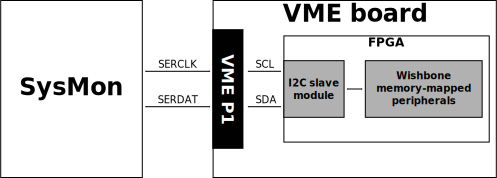
\includegraphics[width=\textwidth]{fig/sys}}
  \caption{Typical system for the \textit{wb\_i2c\_bridge} module}
  \label{fig:sys}
\end{figure}

%==============================================================================
% SEC: Instantiation
%==============================================================================
\section{Instantiation}
\label{sec:instantiation}

The ports of the \textit{wb\_i2c\_bridge} module are shown in Table~\ref{tbl:ports}.
The I$^2$C signals should be connected to tri-state ports, as shown in
Figure~\ref{fig:i2c-ports}; Wishbone slaves should be connected to the
Wishbone master interface ports, prefixed with \textit{wbm}.

\begin{table}[hbtp]
  \caption{Ports of \textit{wb\_i2c\_bridge} module}
  \label{tbl:ports}
  \centerline
  {
    \begin{tabular}{l c p{.6\textwidth}}
    \hline
    \multicolumn{1}{c}{\textbf{Port}} & \textbf{Size} & \multicolumn{1}{c}{\textbf{Description}} \\
    \hline
    clk\_i       &  1 & Clock input \\
    rst\_n\_i    &  1 & Active-low reset input \\
    sda\_en\_o   &  1 & SDA line output tri-state enable \\    
    sda\_i       &  1 & SDA line input \\
    sda\_o       &  1 & SDA line output \\
    scl\_en\_o   &  1 & SCL line tri-state enable \\
    scl\_i       &  1 & SCL line input \\
    scl\_o       &  1 & SCL line output \\
    i2c\_addr\_i &  7 & I$^2$C slave address on ELMA I$^2$C bus \\
    tip\_o       &  1 & Transfer In Progress \newline
                        '1' -- I$^2$C address sent by SysMon matches that of the I$^2$C slave \newline
                        '0' -- after transfer has completed and I$^2$C slave is idle \\
    err\_p\_o    &  1 & Error bit, high for one \textit{clk\_i} cycle when the Wishbone address
                        the SysMon tries to access is invalid \\
    wdto\_p\_o   &  1 & FSM watchdog timer time-out, high for one \textit{clk\_i} cycle when
                        the FSM watchdog has timed-out \\
    wbm\_stb\_o  &  1 & Wishbone data strobe output \\
    wbm\_cyc\_o  &  1 & Wishbone valid cycle output \\
    wbm\_sel\_o  &  4 & Wishbone byte select output \\
    wbm\_we\_o   &  1 & Wishbone write enable output \\
    wbm\_dat\_i  & 32 & Wishbone data input (to master) \\
    wbm\_dat\_o  & 32 & Wishbone data output (from master) \\
    wbm\_adr\_o  & 32 & Wishbone address output \\
    wbm\_ack\_i  &  1 & Wishbone acknowledge signal input \\
    wbm\_rty\_i  &  1 & Wishbone retry signal input \\
    wbm\_err\_i  &  1 & Wishbone error signal input \\
    \hline
    \end{tabular}
  }
\end{table}

\begin{figure}[h]
  \centerline{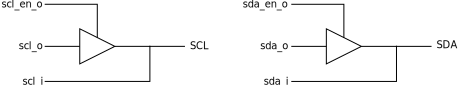
\includegraphics[width=.75\textwidth]{fig/i2c-ports}}
  \caption{I$^2$C port external connections}
  \label{fig:i2c-ports}
\end{figure}

%\begin{table}[h]
%  \caption{Wishbone datasheet of \textit{wb\_i2c\_bridge} module}
%  \label{tbl:wb-ds}
%  \centerline
%  {
%    \begin{tabular}{p{.4\textwidth} p{.43\textwidth}}
%    \hline
%    \multicolumn{1}{c}{\textbf{Description}} & \multicolumn{1}{c}{\textbf{Specification}} \\
%    \hline
%    General description           & ELMA elma-prot to Wishbone bridge \\
%    Supported cycles              & Master, read/write \\
%    Data port, size               & 32-bit \\
%    Data port, granularity        & 32-bit \\
%    Data port, max. operand size  & 32-bit \\
%    Data transfer ordering        & Little-endian \\
%    Data transfer sequencing      & Undefined     \\
%    Supported signal list and
%    cross-reference to equivalent
%    Wishbone signals              & wbm\_stb\_o -- STB\_O \newline
%                                    wbm\_cyc\_o -- CYC\_O \newline
%                                    wbm\_sel\_o -- SEL\_O \newline
%                                    wbm\_we\_o  -- WE\_O  \newline
%                                    wbm\_dat\_i -- DAT\_I \newline
%                                    wbm\_dat\_o -- DAT\_O \newline
%                                    wbm\_adr\_o -- ADR\_O \newline
%                                    wbm\_ack\_i -- ACK\_I \newline
%                                    wbm\_rty\_i -- RTY\_I \newline
%                                    wbm\_err\_i -- ERR\_I \\
%    ERR\_I signal behaviour       & i2c\_err\_o set \\
%    \hline
%    \end{tabular}  
%  }
%\end{table}

%==============================================================================
% SEC: Testing
%==============================================================================
\section{Testing the \textit{wb\_i2c\_bridge} module}
\label{sec:testing}

After proper synthesis and download to the FPGA, a Telnet or serial connection
should be made to the SysMon board. Commands can then be sent to the boards via
the SysMon. The two commands relevant for this basic test are \textit{readreg}
and \textit{writereg}. These and other commands relevant for accessing board
registers are outlined in Section~\ref{sec:elma-prot-cmds}.

The example below shows how to connect to an ELMA crate at IP address 1.2.3.4,
obtaining the value of a register at address 0x10 in a board in VME slot 2,
writing the hex value 0x1234 to the same register and reading it back to check for
proper modification.

\begin{verbatim}
$ telnet 1.2.3.4
Trying 1.2.3.4...
Connected to 1.2.3.4.
Escape character is '^]'.
login:user
password:**********
%>readreg 2 10
 Read Data: 00ABCDEF
%>writereg 2 10 1234
 Done!
%>readreg 2 10
 Read Data: 00001234
\end{verbatim}

%==============================================================================
% SEC: Protocol
%==============================================================================
\section{Data transfer protocol}
\label{sec:elma-prot}

%------------------------------------------------------------------------------
\subsection{Protocol details}
\label{sec:elma-prot-prot}

The VME backplane provides two serial lines (\textit{SERCLK} and \textit{SERDAT})
on the P1 connector. These lines can be used to access boards placed in a VME
slot to control them, in cases where the VME interface is not implemented.
Using I$^2$C as a low-level protocol and the higher-level protocol defined here,
the bytes of a register can be read from or written to a VME board.

Figure~\ref{fig:sysmon-wr} shows a write operation from the SysMon to a VME
board. The process starts with the control byte, containing the board's
I$^2$C slave address and the read/write bit cleared, indicating an 
I$^2$C write. After the slave's ACK, the following two bytes send the 
12-bit register address in little-endian order (most significant byte first). 
After the address has been acknowledged, the following four I$^2$C transfers 
are used to transmit the 32-bit data to be written to the board register.
Data transmission occurs in big-endian order (least significant byte first).

\begin{figure}[h]
  \centerline{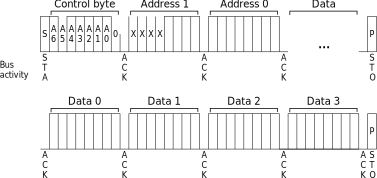
\includegraphics[width=.9\textwidth]{fig/sysmon-wr}}
  \caption{SysMon write operation}
  \label{fig:sysmon-wr}
\end{figure}

\begin{figure}[h]
  \centerline{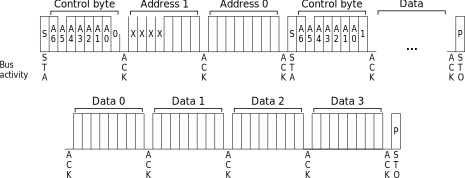
\includegraphics[width=\textwidth]{fig/sysmon-rd}}
  \caption{SysMon read operation}
  \label{fig:sysmon-rd}
\end{figure}

A read transfer (Figure~\ref{fig:sysmon-rd}) from a VME board is similar 
to the write transfer. The differences lie in the retransmission of the
control byte after the register address, this time with the read/write
bit set, to indicate an I$^2$C read. Following the ACK from the slave,
the transfer direction changes and the SysMon will read the four data
bytes sent by the VME board. As with the write transfer, the data bytes
are sent by the VME board in big-endian order.

%------------------------------------------------------------------------------
\subsection{Access commands}
\label{sec:elma-prot-cmds}

In order to send data to a VME board, a user connects to the SysMon via Telnet
and sends commands which the SysMon translates into I$^2$C accesses as outlined
in the previous section. The commands Telnet commands to send to the SysMon are
shown in Table~\ref{tbl:cmds}.

\begin{table}[h]
  \caption{SysMon Telnet commands for I$^2$C access}
  \label{tbl:cmds}
  \centerline
  {
    \begin{tabular}{l p{.6\textwidth}}
    \hline
    \multicolumn{1}{c}{\textbf{Command}}   & \multicolumn{1}{c}{\textbf{Description}} \\
    \hline
    writereg \textit{slot addr val}        & Writes the \textit{hex} value \textit{val} to hex address
                                             \textit{addr} of board in slot number \textit{slot} \\
    writemregs \textit{slot addr v1 .. v8} & Similar to the \textit{writereg} command, but allows writing up to
                                             eight different values to the same Wishbone register. The values
                                             are given in hexadecimal format and are separated by spaces \\
    readreg \textit{slot addr}             & Returns the value of register at hex address \textit{addr} of
                                             board in slot number \textit{slot} \\
    \hline
    \end{tabular}
  }
\end{table}

One noteworthy subject here is the \textit{writemregs} command. This command allows
writing more up to eight words to the same Wishbone register. It is useful
when one wants to use a Wishbone register as a proxy for accessing an on-board
peripheral where large amounts of data are to be written. An external memory is a
good example of such a peripheral.

\begin{figure}
  \centerline{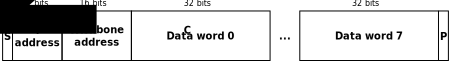
\includegraphics[width=\textwidth]{fig/writemregs}}
  \caption{SysMon write using \textit{writemregs}}
  \label{fig:writemregs}
\end{figure}

In principle, the \textit{writemregs} is a \textit{writereg} with multiple data words
packed together, as outlined in Figure~\ref{fig:writemregs}. In this figure, each data word
is split in four bytes as outlined in Figure~\ref{fig:sysmon-wr}, with an ACK sent by
the VME board after every byte.

As Figure~\ref{fig:writemregs} shows, the data words are sent in little-endian order,
word 0 is sent first, followed by word 1 and so forth, until word 7.

\begin{figure}[h]
  \centerline{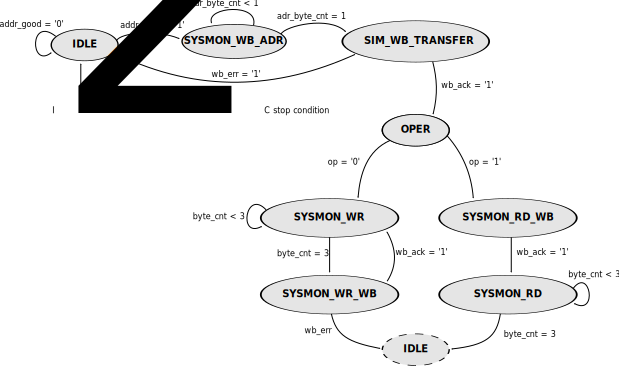
\includegraphics[width=\textwidth]{fig/fsm}}
  \caption{Main FSM of \textit{wb\_i2c\_bridge} module}
  \label{fig:fsm}
\end{figure}

%==============================================================================
% SEC: Implem
%==============================================================================
\section{Implementation}
\label{sec:implem}

In order to perform low-level I$^2$C transfers, the \textit{gc\_i2c\_slave} module
is instantiated and used within the \textit{wb\_i2c\_bridge} module. The outputs
of the \textit{gc\_i2c\_slave} module  are used as controls for an eight-state finite
state machine (FSM), a simplified version of which is shown in Figure~\ref{fig:fsm}.
Table~\ref{tbl:fsm} also lists the states of the FSM.

Where the SysMon appears in the state names, it indicates what the SysMon action is.
For example, if the state of the FSM is \textit{SYSMON\_WR}, this means the SysMon
is writing and the \textit{wb\_i2c\_bridge} is reading.

\begin{table}[h]
  \caption{States of \textit{wb\_i2c\_bridge} FSM}
  \label{tbl:fsm}
  \centerline
  {
    \begin{tabular}{l p{.7\textwidth}}
    \hline
    \multicolumn{1}{c}{\textbf{State}} & \multicolumn{1}{c}{\textbf{Description}} \\
    \hline
    IDLE            & Wait for the \textit{gc\_i2c\_slave} module to receive the I$^2$C
                      address and go to \textit{WB\_ADR} \\
    WB\_ADR         & Shift in the two address bytes sent via I$^2$C and go to
                      \textit{OPER} \\
    OPER            & Check the \textit{op\_o} output of the \textit{gc\_i2c\_slave} module.
                      If '1', go to \textit{SYSMON\_RD\_WB} state (SysMon is reading from
                      \textit{wb\_i2c\_bridge}), otherwise continue shifting in bytes (SysMon
                      writing to \textit{wb\_i2c\_bridge}) \\
    SYSMON\_WR      & Continue reading up to four bytes sent by the SysMon and go to 
                      \textit{SYSMON\_WR\_WB}\\
    SYSMON\_WR\_WB  & Perform a Wishbone write transfer to the register with the address obtained in 
                      \textit{WB\_ADR}. If the transfer is successful, go back to \textit{SYSMON\_WR}
                      to continue receiving register data (useful for the \textit{writemregs} command
                      -- see Section~\ref{sec:elma-prot-cmds}) \\
    SYSMON\_RD\_WB  & Perform a Wishbone read transfer from the address obtained in
                      \textit{WB\_ADR} and go to \textit{SYSMON\_RD} \\
    SYSMON\_RD      & Shift out the four bytes of the Wishbone register when the \textit{gc\_i2c\_slave}
                      module successfully finishes a write \\
    \hline
    \end{tabular}
  }
\end{table}

To better understand how the FSM operates, Figures \ref{fig:sysmon-wr-fsm} and
\ref{fig:sysmon-rd-fsm} can be consulted, where the state of the FSM is shown
during reads and writes from the SysMon.

When the SysMon writes (Figure~\ref{fig:sysmon-wr-fsm}), the
\textit{wb\_i2c\_bridge} module waits in the \textit{IDLE} state until
the I$^2$C address is received, then, while in the \textit{WB\_ADR} state,
it shifts in the Wishbone address. The first byte of the write transfer is shifted
in while in the \textit{OPER} state, followed by the next three bytes while in the
\textit{SYSMON\_WR} state. The register is written to in the \textit{SYSMON\_WR\_WB}
state using a Wishbone write transfer.

To allow for the \textit{writemregs} command, whereby up to eight registers can be
written with one I$^2$C transfer, the FSM goes back to the \textit{SYSMON\_WR} state
if the Wishbone write transfer completed successfully. The FSM will go back into the
\textit{IDLE} state when an I$^2$C stop condition is received, which is sent by
the SysMon after the \textit{writereg} or \textit{writemregs} has been completed.

\begin{figure}[h]
  \centerline{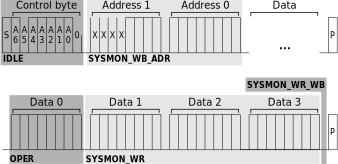
\includegraphics[width=.8\textwidth]{fig/sysmon-wr-fsm}}
  \caption{FSM states when the SysMon writes to the \textit{wb\_i2c\_bridge}}
  \label{fig:sysmon-wr-fsm}
\end{figure}

\begin{figure}[h]
  \centerline{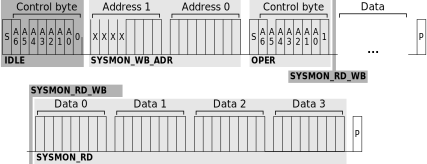
\includegraphics[width=\textwidth]{fig/sysmon-rd-fsm}}
  \caption{FSM states when the SysMon reads from the \textit{wb\_i2c\_bridge}}
  \label{fig:sysmon-rd-fsm}
\end{figure}

When the SysMon reads (Figure~\ref{fig:sysmon-rd-fsm}), the address is shifted in
as in the case of a write. In the case of a SysMon reading from a board,
however, the I$^2$C transfer is restarted and the order is reversed (SysMon starts
reading). Thus, while in \textit{OPER}, the FSM detects a high value on \textit{op\_o}
corresponding to an I$^2$C read transfer, and goes into the \textit{SYSMON\_RD\_WB}
state. The value of the register is read while in this state, and sent via I$^2$C
in the \textit{SYSMON\_RD} state.

Note that on an error in any Wishbone transfer, the FSM goes back to the \textit{IDLE}
state, setting the \textit{err\_p\_o} output for one \textit{clk\_i} cycle.

The design also contains an FSM watchdog component, which resets the main FSM
in case of errors in communication. The watchdog timeout value is configured
via the \textit{g\_wdt\_max} generic and can be calculated as outlined in
Appendix~\ref{app:wdto-calc}.

%==============================================================================
% SEC: Synthesis results
%==============================================================================
\section{Synthesis results}
\label{sec:synth-res}

The synthesis results for the \textit{wb\_i2c\_bridge} design using \textit{xst}
on the Spartan-6 XC6SLX45T are shown in Table~\ref{tbl:synth-res}.

\begin{table}[h]
  \caption{Synthesis results}
  \label{tbl:synth-res}
  \centerline{
  \begin{tabular}{l c c c}
  \hline
  \multicolumn{1}{c}{\textbf{Resource}} & \textbf{Used} & \textbf{Available} & \textbf{\%} \\
  \hline
  Slices          & 94  & 6822  & 1.3 \\
  Slice registers & 168 & 54576 & 0.3 \\
  LUTs            & 188 & 27288 & 0.6 \\
  \hline
  \end{tabular}
  }
\end{table}

%==============================================================================
% Appendix
%==============================================================================
\pagebreak
\begin{appendices}

\section{Watchdog timeout value calculation}
\label{app:wdto-calc}

In order to calculate the maximum watchdog timeout value, the following procedure
should be utilized.

First, the frequency on the I$^2$C communication in ELMA crates is 100~kHz. One
I$^2$C byte transfer always consists in 9 bits (eight bits for data plus one for
acknowledgement). Therefore, one I$^2$C byte is transferred within 90~$\mu$s.

To account for start and stop conditions and to allow for frequency changes on
the bus, one can consider one I$^2$C byte as 10 bits, therefore one I$^2$C
transfer can be considered to take 10~$\mu$s to complete.

Now, taking this into account and the period of the \textit{clk\_i} input,
$T_{clk\_i}$, the number of clock cycles needed to complete one I$^2$C byte transfer
can be calculated as:

\begin{equation}
N_{byte} = \frac{10 {\mu}s}{T_{clk\_i}}
\end{equation}

Within the ELMA crates, a maximum of 35 bytes can be sent through I$^2$C. This
happens when using the \textit{writemregs} command, where one byte is needed
for the I$^2$C address, two for the Wishbone address and a maximum of 32 bytes for
data (8 32-bit registers). Leaving a safety margin, one can calculate the
maximum watchdog timeout value to be the time needed to send 40 bytes via I$^2$C
on the bus:

\begin{equation}
g\_wdt\_max = 40 * N_{byte} = 40 * \frac{10 {\mu}s}{T_{clk\_i}}
\end{equation}

\end{appendices}

%==============================================================================
% Bibliography
%==============================================================================
\pagebreak
\bibliographystyle{ieeetr}
\bibliography{wb_i2c_bridge}

\end{document}
